\section{Sensor Fusion}
\label{sensor_fusion}

Now, that you've learned the basics of estimation theory, 3D geometry, and some common sensing modalities, it's time to put it into practice and think about how we can use all of these tools together to build an estimator we can use on a real self-driving car. A real self-driving car is typically equipped with many different kinds of sensors such as cameras, LiDAR, IMU, radar units, a GPS or GNSS receiver, and a wheel encoders. All of these sensors give us different types of data at different rates. For example, the IMU might report accelerations and angular velocities 200 times per second, while the LiDAR completes a full scan only 20 times per second.Thus, we want to think how we are going to talk about how we can combine all the different information to get the best possible estimate of the vehicle state. 
This process is called \textbf{sensor fusion} and it's one of the most important techniques for self-driving cars. However, in order to do sensor fusion, we also need to calibrate our sensors to ensure that the sensor models are accurate and so that we know how the reference frames of all of the sensors are related to each other. We also need to discuss what happens when one or more sensors fails. 

Thus, in the first section, we will have a bird's-eye view of some practical considerations we should take into account when designing systems for self-driving cars. 

\begin{itemize}
\item Sensor fusion and calibration
\item Accuracy requirements
\item Localization failures 
\item How to cope with parts of the environment that are moving and changing around us
\end{itemize}


\subsection{Why do we need sensor fusion?}
\label{why_do_we_need_sensor_fusion}

 If we have a car that is equipped with a number of different sensors, what we would like to do is figure out how to combine all of this different information to get the best possible estimate of the vehicle state. It might seem like a daunting task to fuse all of this data, but in fact, we already have the tools to do this. For example, we have already discussed the extended Kalman filter to combine all of the sensor data into a single consistent estimate of the vehicle state. However, in order to do sensor fusion, we first need to know some things about our sensors and how they are configured on board the vehicle. This is because our sensor models might depend on parameters that are specific to the car or to the sensor itself. A good example of this is using wheel encoders to measure the forward speed of the car. 

A wheel encoder measures the angular velocity of the axle. If we want to use that to get the forward velocity of the vehicle, we also need to know the radius of a tire. Another thing we need to know about the vehicle is the pose or position and orientation of each sensor relative to the vehicle reference frame. Because we are combining information from sensors located in different places, we need to know how to transform all of the measurements so they are expressed in a common reference frame. Finally, we need to think about how well our sensor measurements are synchronized so that we can fuse them all properly. 

Intuitively, you might expect that directly combining a LiDAR scan you just received with a GPS measurement you received, say, five seconds ago, will not produce as good of a result as if the LiDAR scan and the GPS measurement were taken at the same time. So, the more accurately you can synchronize your sensors, the better your state estimate will be. A part of this involves determining the time offset between when the sensor records a measurement and when the estimator receives it for processing. All of these factors are critical forms of calibration.  How accurate does a estimator need to be for a self-driving car to drive safely on the road? It depends on several factors like

\begin{itemize}
\item The size of the car
\item The width of the lanes
\item The density of traffic
\end{itemize}

 In order to get a ballpark estimate, you might consider the margin of error available for a task leak lane keeping. A typical car is about 1.8 meters wide, an average highway 
lane might be about three meters wide, give or take. So, our estimator would need to be good enough to position the car within 60 centimeters or so on either side of the lane. 
This is assuming we know exactly where the lanes are and that there is no traffic. For comparison, an optimistic range for GPS accuracy is between one and five meters depending on the specific hardware, the number of satellites that are visible, and other factors. Clearly, therefore, GPS alone is not enough even for lane keeping. This is one important reason why we'll need to combine information from many different sensors. 

Another question that pops up is how fast we need to update the vehicles states whether the car can react to rapidly changing environments or unexpected events? This all depends on what kind of environment the car is operating in. Imagine that you are driving a car with your eyes closed, and you open your eyes exactly once every second to take a look at what is around you and make some adjustments. This corresponds to an update rate of one hertz. For driving down a street country road with no traffic in sight, maybe you'll feel relatively safe doing this. But what if you are driving through a busy city intersection with dozens of other cars, and buses, and cyclists, and pedestrians around you? You would probably feel much less safe opening your eyes once a second. As a rule of thumb, an update rate of 15 hertz to 30 hertz is a reasonable target for self-driving. But of course, there's a trade-off to think about here. A self-driving car will only have so much on-board computing power available and the computer will need to juggle many different processes like control and path planning and perception in addition to state estimation. Moreover, the total amount of compute power available on board may be limited by restrictions on how much power the computer is actually allowed to consume. Produce state estimation with fixed computational resources, there is a trade-off between how complicated our algorithms can be and the amount of time are allowed to spend computing a solution. It is up to the engineer to decide where the car is going to be on this trade off curve. 

Even if we had a fast and accurate estimation algorithm, there are going to be cases where our localization might fail. How could this happen? We might, for example, have one or more of our sensors report bad data or maybe even fail entirely. A good example of this is GPS which doesn't work at all in tunnels and which can have a difficult time coping with reflected signals in cities with a lot of tall buildings. We might also encounter errors in our state estimation algorithm itself. For example, if we're using an extended common filter with a highly nonlinear sensor model, we might find that the inherent linearization error in the estimator means that we can lose accuracy in our state estimate even though the estimator is pretty confident in its output. Or maybe, our estimator is not very confident at all. Thinking back to the Kalman filter equations, you might remember that the uncertainty in our state grows as we propagate forward through the motion model and it only shrinks once we incorporate outside observations from LiDAR or GPS for example. If our LiDAR is broken and we are driving in a tunnel without GPS, how long can we rely on an IMU and a motion model before our estate uncertainty grows too large and it is no longer safe to drive? We need thus strategies for detecting and coping with localization failures like these. Finally, we need to think about the world the car lives in. 
For the most part, we have developed our models for sensors like LiDAR under the assumption that the world is static and unchanging. Of course, in reality, the world is always moving and changing. 

For example, other cars, pedestrians, and cyclists are probably moving. Lighting changes over the course of a day and even the geometry of the world can change with the seasons. 
One of the big challenges for self-driving cars is finding ways to account for these kinds of changes, whether by modeling them or by finding ways of identifying and ignoring objects that violate our assumptions. 

All in all, state estimation in practice will typically rely on sensor fusion to combine information from many different kinds of sensors, like IMUs, LiDAR, cameras, and GPS or GNSS receivers. In order for sensor fusion to work as intended, we need to calibrate the sensors by determining the parameters of our sensor models. The relative positions and orientations of all of the sensors and any differences in polling times. We also need to consider trade-offs between speed and accuracy in our algorithms which may be different depending on the type of self-driving car. Ask yourself, how accurately do I need to know the vehicle state and how often do I need to update it for my particular use case? Finally, we need to think about how to safely cope with localization failures and aspects of the world that do not conform to our assumptions such as moving objects. 




\subsection{Multisensor Fusion}
\label{multisensor_fusion}

The previous section gave a brief outline on the why we need sensor fusion.  In this section,
we will derive an error state extended Kalman Filter that
estimates position, velocity, and orientation of a self-driving car using an IMU, a GNSS receiver,
and a LIDAR. Although we'll make some simplifications, the basic structure
of our pipeline will resemble one used in a modern self-driving vehicles. 

Before we dive into
the algorithm details, it's always useful to take a step back and ask why we use these sensors and can we do something
more simple? In our case, we'll be using an IMU with a GNSS receiver and a LIDAR for several reasons. 

\begin{itemize}
\item First, whenever we fuse information for the purpose of state estimation, one important factor
to consider is whether or not the errors from different sensors will be correlated. In other words,
if one fails is the other likely to fail as well. In this case, all three of our sensors use different measurement
methods and are unlikely to fail for the same reason. 
\item Second, we should try our best to choose sensors that are complimentary in nature. In our case, the IMU acts as a high-rate
smoother of GPS or GNSS position estimates. GNSS data can mitigate errors that are due to IMU drift. It's also possible to use wheel odometry for this purpose. 
\end{itemize}

In this section, we will stick to IMUs as they can provide full position
and orientation information in three-dimensions, whereas wheel odometry is limited to two dimensions. Finally, LIDAR
can compliment GNSS information by providing very accurate position estimates within a known map and in sky obstructed locations. 
Conversely, GNSS can tell LIDAR which map to use when localizing. 




For the purposes of EKF state estimation, we can implement either what's called a loosely coupled estimator or a
tightly coupled one. In a tightly coupled EKF, we use the raw pseudo range and point cloud measurements from our GNSS and LIDAR
as observations. In a loosely coupled system, we assume that this data has already been preprocessed to produce a noisy
position estimate. Although the tightly coupled approach can lead to more accurate localization, it's often tedious
to implement and requires a lot of tuning. For this reason, we will implement a loosely coupled EKF here. 

Figure \ref{ekf_sensor_fusion} shows a graphical representation
of our system. We will use the IMU measurements as noisy inputs to
our motion model. This will give us our predicted state which will update every time we have an IMU measurement, this can happen hundreds
of times a second. At a much slower rate, we'll incorporate GNSS and LIDAR measurements whenever they become available, say once a second
or slower, and use them to correct our predicted state. 

\begin{figure}[!htb]
\begin{center}
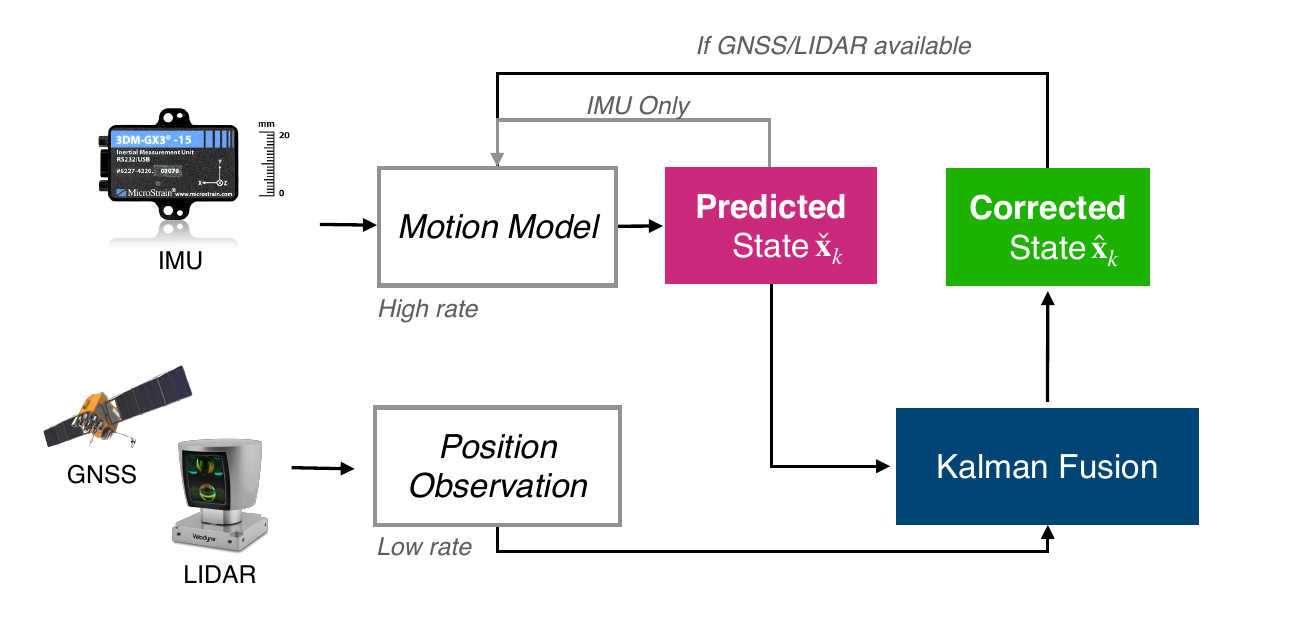
\includegraphics[scale=0.280]{img/sensor_fusion/ekf_sensor_fusion.jpeg}
\end{center}
\caption{Block diagram of the sensor fusion process .}
\label{ekf_sensor_fusion}
\end{figure}

So, what is our state? For our purposes, we will use a ten-dimensional
state vector that includes a 3D position, a 3D velocity, any 4D unit
quaternion that will represent the orientation of our vehicle with respect to a navigation frame. 

\begin{equation}
\mathbf{x}_k = 
\begin{bmatrix}
\mathbf{p}_k \\
\mathbf{v}_k \\
\mathbf{q}_k 
\end{bmatrix} \in R^{10}
\end{equation}


We will assume that IMU outputs specific forces and rotational rates in the sensor frame and combine them into a single
input vector $\mathbf{u}$. 

\begin{equation}
\mathbf{u}_k =
\begin{bmatrix}
\mathbf{f}_k \\
\boldsymbol{\omega}_k
\end{bmatrix} \in R^6
\end{equation}

It is also important to point out that we are not going to track accelerometer
or gyroscope biases. These are often put into the state vector, estimated, and then subtracted off of the our IMU
measurements. For clarity, we will emit them here and assume our IMU measurements
are unbiased. Our motion model for the position, velocity, and orientation
will integrate the proper accelerations and rotational rates
from our IMU. 

The motion model involves position, velocity and orientation updates. The position updates look like this. 

\begin{equation}
\mathbf{p}_k = \mathbf{p}_{k-1} + \Delta t \mathbf{v}_{k-1} + \frac{(\Delta t)^2}{2}(\mathbf{C}_{ns}\mathbf{f}_{k-1} - \mathbf{g}) 
\end{equation}

Next is the velocity update,


\begin{equation}
\mathbf{v}_k = \mathbf{v}_{k-1} + \Delta t (\mathbf{C}_{ns}\mathbf{f}_{k-1} - \mathbf{g}) 
\end{equation}

and the quaternion update. 

\begin{equation}
\mathbf{q}_k = \boldsymbol{\Omega} (\mathbf{q}(\boldsymbol{\omega}_{k-1} \Delta t))\mathbf{q}_{k-1} 
\end{equation}

We will need to use a bunch of definitions as shown below. 


\begin{equation}
\mathbf{q}(\boldsymbol{\theta})  = 
\begin{bmatrix}
\sin(\frac{|\boldsymbol{\theta}|}{2}) \\
\frac{\boldsymbol{\theta}}{|\boldsymbol{\theta}|}\cos(\frac{|\boldsymbol{\theta}|}{2})
\end{bmatrix} 
\end{equation}

\begin{equation}
\boldsymbol{\Omega}( 
\begin{bmatrix}
q_w \\
\mathbf{q}_{v}
\end{bmatrix}) = q_w \mathbf{I} + 
\begin{bmatrix}
0 & - \mathbf{q}_{v}^T \\
\mathbf{q}_{v} & \mathbf{q}_{v} 
\end{bmatrix}
\end{equation}

Remember that our quaternion will keep track of
the orientation of our sensor frame $S$ with respect to
our navigation frame $n$. Because of the orientation parameters, which we express as
a rotation matrix, our motion model is nonlinear. In order to use it in our EKF, we'll need to linearize
it with respect to some small error or perturbation about
the predicted state. To do this, we will define an error state

\begin{equation}
\delta \mathbf{x}_k = 
\begin{bmatrix}
\delta \mathbf{p}_k \\
\delta \mathbf{v}_k \\
\delta \boldsymbol{\phi}_k
\end{bmatrix} \in R^9
\end{equation}

where $\delta \boldsymbol{\phi}$ is a three by one orientation error. Using this state,
we can derive error dynamics with the appropriate Jacobians. 

\begin{equation}
\delta \mathbf{x}_k = \mathbf{F}_{k - 1} \delta \mathbf{x}_{k-1} + \mathbf{L}_{k-1} \mathbf{n}_{k-1}
\end{equation}

where

\begin{equation}
\mathbf{F}_{k-1} = 
\begin{bmatrix}
\mathbf{I} & \mathbf{I}\Delta t & \mathbf{0} \\
\mathbf{0} & \mathbf{I} & - [\mathbf{C}_{ns}\mathbf{f}_{k-1}]\Delta t \\
\mathbf{0} & \mathbf{0} & \mathbf{I} 
\end{bmatrix}
\end{equation}

\begin{equation}
\mathbf{L}_{k-1} = 
\begin{bmatrix}
\mathbf{0} & \mathbf{0} \\
\mathbf{I} & \mathbf{0}  \\
\mathbf{0} & \mathbf{I} 
\end{bmatrix}
\end{equation}

\begin{equation}
\mathbf{n}_{k} \sim N(\mathbf{0}, \mathbf{Q}_k) 
\end{equation}

where

\begin{equation}
\mathbf{Q}_{k} = (\Delta t)^2
\begin{bmatrix}
\sigma_{acc}^2 & 0  \\
0 & \sigma_{gyro}^2 
\end{bmatrix},
\mathbf{I} =
\begin{bmatrix}
1 &  0 & 0 \\
0 &  1 & 0 \\
0 &  0 & 1  
\end{bmatrix}
\end{equation}

For our measurement model, we will use a very
simple observation of the position plus some additive Gaussian noise. 

\begin{equation}
\mathbf{y}_k = h(\mathbf{x}_k) + \boldsymbol{\nu}_k = \mathbf{p}_k + \boldsymbol{\nu}_k, \boldsymbol{\nu}_k \sim N(\mathbf{0}, \mathbf{R}_{GNSS})
\end{equation}

We will define a covariance $\mathbf{R}_{GNSS}$, for the GNSS
position noise. We do similarly for the LiDAR

\begin{equation}
\mathbf{y}_k = h(\mathbf{x}_k) + \boldsymbol{\nu}_k = \mathbf{p}_k + \boldsymbol{\nu}_k, \boldsymbol{\nu}_k \sim N(\mathbf{0}, \mathbf{R}_{LIDAR})
\end{equation}

\begin{framed}
\theoremstyle{remark}
\begin{remark}{\textbf{Coordinate Transformations}}

It is important here
to note that we have assumed that our LIDAR and GNSS will supply
position measurements in the same
coordinate frame. 
\end{remark}
\end{framed}

In a realistic implementation, the GNSS position estimates may serve as a way to select a known map against which
the LIDAR data can then be compared. 

\subsection{The Extended Kalman Filter}

With these definitions in mind, we can now describe our extended
Kalman filter. Our filter will loop every time an IMU measurement occurs. We will first use the
motion model to predict a new state based on our last state. The last state may be a fully corrected state or one that was
also propagated using the motion model only depending on whether or not we received a GNSS or
LIDAR measurement at the last time step. Next, we will propagate the state uncertainty through our linearized
motion model. Again, accounting for whether or not our previous state was corrected or uncorrected. At this point,
if we do not have any GNSS or LIDAR measurements available, we can repeat
steps one and two. If we do, we will first compute the Kalman gain that is appropriate for the given observation, we will then compute
an error state that we will use to correct our predicted state. 

This error state is based on the product of
the Kalman gain and the difference between the predicted and
observed position. We will then correct our predicted state
using our error state. This correction is
straightforward for position and velocity, but some more
complicated algebra is required to correct
the quaternion. We will need
this special update because the quaternion is a constrained
quantity that is not a simple vector. 
Finally, we'll update our state covariants in the usual way. 

In summary, our algorithm is

\begin{enumerate}
\item Update state with IMU inputs according to
\begin{equation}
\check{\mathbf{p}}_k = \mathbf{p}_{k-1} + \Delta t \mathbf{v}_{k-1} + \frac{(\Delta t)^2}{2}(\mathbf{C}_{ns}\mathbf{f}_{k-1} - \mathbf{g}) 
\end{equation}
\begin{equation}
\check{\mathbf{v}}_k = \mathbf{v}_{k-1} + \Delta t (\mathbf{C}_{ns}\mathbf{f}_{k-1} - \mathbf{g}) 
\end{equation}
\begin{equation}
\check{\mathbf{q}}_k = \boldsymbol{\Omega} (\mathbf{q}(\boldsymbol{\omega}_{k-1} \Delta t))\mathbf{q}_{k-1} 
\end{equation}
\item  Propagate uncertainty according to 
\begin{equation}
\check{\mathbf{P}}_k = \mathbf{F}_{k-1}\check{\mathbf{P}}_{k-1} \mathbf{F}_{k-1}^T + \mathbf{L}_{k-1}\mathbf{Q}_{k-1}\mathbf{L}_{k-1}^T
\end{equation}
\item  If GNSS or LIDAR position available:
\begin{enumerate}
\item  Compute Kalman gain
\begin{equation}
\mathbf{K}_k = \check{\mathbf{P}}_k\mathbf{H}_{k}^T(\mathbf{H}_{k}\check{\mathbf{P}}_k\mathbf{H}_{k}^T + \mathbf{R})^{-1}, 
\end{equation}
$\mathbf{R}$ is one of $\mathbf{R}_{GNSS}$ or $\mathbf{R}_{LIDAR}$ 
\item  Compute error state
\begin{equation}
\delta\hat{\mathbf{p}}_k = \mathbf{K}_k(\mathbf{y}_k - \check{\mathbf{p}}_k) 
\end{equation}
\item Correct predicted state
\begin{equation}
\hat{\mathbf{p}}_k = \check{\mathbf{p}}_k +\delta \mathbf{p}_k 
\end{equation}
\begin{equation}
\hat{\mathbf{v}}_k = \check{\mathbf{v}}_k +\delta \mathbf{v}_k 
\end{equation}
\begin{equation}
\hat{\mathbf{q}}_k = \boldsymbol{\Omega}(\mathbf{q}(\delta \boldsymbol{\phi}))\check{\mathbf{q}}_k 
\end{equation}
\item Computed corrected covariance
\begin{equation}
\hat{\mathbf{P}}_k = (\mathbf{I} - \mathbf{K}_{k} \mathbf{H}_{k})\check{\mathbf{P}_{k}} 
\end{equation}
\end{enumerate}
\end{enumerate}


\begin{framed}
\theoremstyle{remark}
\begin{remark}{\textbf{Coordinate Transformations}}

$\mathbf{p}_{k-1}, \mathbf{v}_{k-1}, \mathbf{q}_{k-1}$ can be either corrected or uncorrected depending on whether or not there was
a GNSS/LIDAR measurement at time step $k-1$. 
\end{remark}
\end{framed}

Let us review a few of the assumptions we have made when putting
our pipeline together. We used a loosely-coupled extended Kalman
Filter framework to fuse inertial measurements from an IMU together with position measurements
from a GNSS receiver and LIDAR. We assume that the GNSS and LIDAR provided us with position estimates in the same coordinate frame which requires
some preprocessing, but is possible to do in a realistic
implementation. Second, we did not account for accelerometer or gyroscope biases in our IMU measurements. This simplified
our algebra but is not a realistic assumption. Luckily, if you follow along with what
we have done here, adding biases is not insignificant leap. Next, we did not discuss Filter State
initialization. This is often taken to be some known state at the start of the localization process. Finally, we also assumed that our
sensors were all spatially and temporally aligned. We assumed that
our sensors were calibrated in the sense that we did not worry about varying time steps or how we can get several sets of
measurements all aligned into one coordinate frame. Performing
this latter step is a very important part of constructing an accurate localization pipeline. 

\subsection{Sensor calibration}
\label{sensor_calibration}
 

\section{Questions}
\label{questions_sensor_fusion}

\subsection{Assignements}
\label{assignements_sensor_fusion}



